% 9 variables in here:
% h_1 = 1000.0, h_2 = 1000.0, h_3 = 1000.0, ux_1 = 4.0, ux_2 = -2.0, ux_3 = 2.0, uy_1 = -2.0, uy_2 = 4.0, uy_3 = 1.0
\begin{figure}[h!]
\centering
  \quad \subfloat[] {
    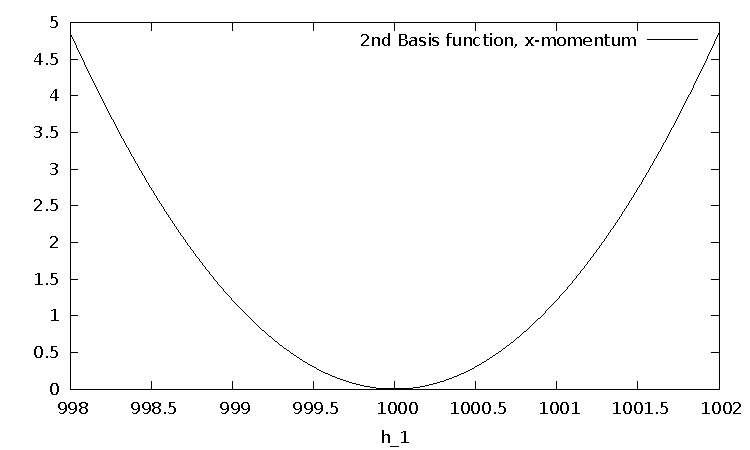
\includegraphics[scale=\zoomfactor]{{{magnitude_1000_momentums/y_1000.0_1000.0_4.0_-2.0_2.0_-2.0_4.0_1.0f02}}}
  }
\caption{}
\label{fig:magnitude_1000_momentums}
\end{figure}

%%% Local Variables:
%%% TeX-master: "../results.tex"
%%% End:
